% Second chapter
\chapter{Economic engineering with analytical mechanics}
\label{chap:ee}
Economic engineering is built on analogies between (macro)economic theory and common engineering disciplines such as thermodynamics, circuit theory and (classical) mechanics\footnote{as opposed to more recent theories in relativistic mechanics and quantum mechanics}. Escpecially for the latter, a rich variety of useful analogues can be devised. There are two common classses of interpretations mechanics: \emph{analytical mechanics} including the formulations by Joseph-Louis Lagrange and sir William Rowan Hamilton, and \emph{vectorial mechanics}, better known as \emph{Newtonian mechanics}. The former variant is usually preferred in the field of engineering whereas the analytical mechanics are more common in physics due to their mathematical elegance and powerful theoretical foundation. Likewise, the theory of economic engineering can be approached in two similar ways. Usually the `Newtonian' approach is given the most attention, but in the case of this work the energy-based approach will prove to be more useful, which is why it is the subject of this discussion. This discussion will mostly pertain to `regular' economic systems, but it is the underlying aspiration of this research that these formal methods will allow to establish a sound framework for financial systems as well.

Analytical mechanics, more specifically \emph{Lagrangian} and \emph{Hamiltonian} mechanics, are established around the definition of special state functions, respectively called the Lagrangian \(\lag\) and the Hamiltonian \(\ham\). As per usual, Lagrangian mechanics will be introduced first, for it has the most intuitive explanation. Then, a more formal approach allows to (Legendre) transform the discussion into one of Hamiltonian mechanics. 

In this chapter, frequent analogies will be made between mechanics and economics; as such, the idea is to have the `normal text' pertain mostly to the discussion of classical mechanics, and to provide the analogies in special `boxes' like so:
\begin{econ}{Example}
    An analogy between economics and classical mechanics.
\end{econ}
The reason for this particular choice of layout is twofold: first, it allows to make a sharp distinction between the older, extremely rigorous theory of classical mechanics and the novel approach of economic engineering: many ideas and propositions are still tentative (especially in the realm of classical mechanics) as the field of economic engineering matures. Secondly, it allows for easier reference as to not obscure the economic analogies (which are arguably the most important aspects of this chapter) with the highly theoretical discussion of analytical mechanics.
\section{Economic engineering}
The discipline of `economic engineering' is a very new one. The theoretical foundations have been developed over the past years at the Delft Center of Systems and Control primarily by prof. em. dr. ir. Mendel, combined with the contributions of several theses that have been recently written about the subject. The purpose of economic engineering is to use tools from various engineering disciplines and physics to improve the predictive power of (macro)economic models. The core idea is to extend `domain-neutral' modeling techniques such as bond graph modeling \cite{Karnopp2012} that are built on analogies between mechanical, electrical, hydraulic, ... systems to economic systems as well. Hence, one attempts to give an economic interpretation to a generalized mass (I-element), generalized spring (C-element) and generalized damper (R-element). The idea is that this consistent engineering approach leads to actual \emph{predictive} models that provide much richer insights than the `stylized facts' from macroeconomy or, on the other end of the spectrum, the `black-box' econometric models that have lost all interpretative value. Indeed, applied economic engineering pursues \emph{grey-box} modeling instead, as is most common in traditional engineering models \cite{Kruimer2021}. Some analogies between mechanical, electrical and economic systems are listed in \cref{tab:analogies} to merely for the sake of illustration; a thorough motivation for each of them will be given in the following section. \Cref{tab:analogies} provides some examples of the analogies that are used within economic engineering. In general, their meaning is not as specific as given here and this table applies only to the most elementary cases. 
\begin{table}[h]
    \centering
    \caption{Some examples of the analogies that are used in the application of economic engineering. The theory behind bond-graph modeling defines a generalization of the mechanical concepts of displacement, velocity, momentum and effort and applies these to electrical, thermodynamic, hydraulic, ... systems too \cite{Karnopp2012}.}
    \label{tab:analogies}
    \begin{tabular}{cccc}
        \toprule
        \textbf{General} & \textbf{Mechanical} & \textbf{Electrical} & \textbf{Economic} \\ 
        \midrule
        Displacement & Displacement & Charge & Stock level\\
        Flow & Velocity & Current & Flow of goods \\
        Momentum & Momentum & Flux linkage & Price \\
        Effort & Force & Voltage & Economic want \\
        \midrule
        I-element & Mass & Inductor & Market \\
        C-element & Spring & Capacitor & Storage of goods \\
        R-element & Damper & Resistor & Depreciation / Consumption \\
        \bottomrule
    \end{tabular}
\end{table}
The main theory behind economic engineering is outlined by \citet{Mendel2019}. Some other notable results in the field have been achieved in recent years as well. \citet{Hutters2020b} demonstrated the application of Hamiltonian mechanics to dissipative systems as to include the mechanics of consumption in port-Hamiltonian systems. A formal approach inspired by the theory of thermodynamics was used by \citet{Manders2019} to explain economic growth and productivity. \citet{Kruimer2021} and \citet{VanArdenne2020} used economic engineering bond graph techniques to build extensive models for the U.S. economy and a `generalized' firm (as to improve business valuation techniques).

\section{Lagrangian mechanics}
\subsection{The configuration manifold}
Central to the concept of Lagrangian mechanics is the so-called \emph{configuration space} \(M\), which is an \(n\)-dimensional manifold provided with some parameterization called \emph{generalized coordinates} assembled in the vector \(\gpos\). 
The configuration manifold may just be equal to \(\real^n\), but in more interesting and realistic cases it is often some manifold embedded in \(\real^n\). This is often the result of holonomic constraints, which are constraints that impose a restriction only on the configuration space, but not, for example, on the allowable velocities.
By using the generalized coordinates, one can parameterize all the allowable positions of a system whose motions may occur in a higher-dimensional space with a smaller coordinate set (e.g. the two-dimensional motion of a pendulum can be expressed in a single coordinate due to the constraint imposed by the rigid link).  The crucial insight here is that the constraint forces will never perform any work on the system\footnote{This is known as \emph{D'Alembert's principle}.}; as such, they act always orthogonally to the configuration manifold. This is why, provided that one is succesful in correctly describing this manifold with a suitable coordinate set, the constraint forces need not be taken into account: a  major advantage over Newtonian mechanics. 
\index{configuration manifold}
\index{configuration space}
\index{generalized coordinates}
\index{holonomic}
\index{nonholonomic}

Unfortunately, the pursuit of finding a set of these all-encompassing generalized coordinates is fruitless for some systems, for they cannot possibly be represented in this simple fashion. Luckily, for a certain class of constraints they may be included to constrict the motion of the system nevertheless by means of the \emph{Lagrange multipliers}. They are applicable to holonomic constraints for which it is impractical or nonintuitive to take them into account directly in the parameterization of the configuration manifold, and a restricted class of nonholonomic constraints that can be written in the so-called \emph{Pfaffian} form \cite{Bullo2005}.
\index{Pfaffian form}
\index{Lagrange multipliers}

\begin{figure}[ht]
    \centering
    \begin{tikzpicture}[scale=1.3]
    \draw[->] (0, 0) -- (0, 3) node[anchor=south] {$z$};
    \draw[->] (0, 0) -- (3, 0) node[anchor=west] {$y$};
    \draw[->] (0, 0) -- (-1.5, -1.5) node[anchor=north east] {$x$};
    \filldraw[draw, fill=white, thick, looseness=0.8] 
    (-2, 1) 
    to[bend left] coordinate (q21) (-1, 2.5)
    to[bend left] coordinate (q11) (1.5, 1) 
    to[bend left] coordinate (q22) (1.2, -1.2) 
    to[bend right] coordinate (q12) cycle node[] {$M$};
    
    \path[draw, dashed, name path=q1, looseness=0.4] (q11) to[bend left] (q12); 
    \path[draw, dashed, name path=q2, looseness=0.8] (q21) to[bend left] (q22); 
    \path [name intersections = {of = q1 and q2}];

    \draw[fill=gray!10, fill opacity=0.6] 
    (-1.6, 1.4) 
    --  (-0.6, 2.9) 
    -- (1.4, 1.4) 
    -- (1.6, -0.8) 
    --  cycle ;
    \node at (1.5, 1.8) {$TM_{\vec{x}}$};
    \node[fill=black,circle,inner sep =1pt] (q) at (intersection-1) {};
    \draw[->, thick] (q) -- ++(0.1, 0.4) node[anchor= west] {$\dot{q}_1$};
    \draw[->, thick] (q) -- ++(-0.43, 0.35) node[anchor=south east] {$\dot{q}_2$};
    
\end{tikzpicture}

    \caption{Schematic of a two-dimensional (configuration) manifold $M$ embedded in $\real^3$; the local generalized velocities associated with a point $\vec{x}$ are vectors that live in the tangent space $TM_{\vec{x}}$.}
    \label{fig:conf_mnfold}
\end{figure}

\begin{econ}{Configuration manifold and the economic system}
    In economic engineering, \(\gpos\) has a similar intuitive notion, namely the stock values of various products, which denote the `position' of some economic system. The name `position' may be misleading when intuitively ported to the familiar three-dimensional space; the configuration space usually has less structure such as the absence of a metric or inner product.\\

    Just like in mechanics, the simplest shape the configuration manifold $M$ can take is a simple $n$-dimensional vector space, but more sophisticated cases exist as well. As mentioned, a nontrivial configuration manifold is usually the result of holonomic constraints applied to the system; these constraints have their meaning in economics too.
    For example, when Lagrangian analysis is applied to the analysis of electrical circuits, the generalized coordinates naturally reflect Kirchoff's current laws (what comes in must go out); as they provide simple constraints to the current in each part of the circuit. An intuitive extension can be made to economics, where the flow of goods is often subject to a Kirchoff-type law as well, especially when considering supply chains or transport. \\
    
    A simple example in economic engineering might be a market with a supplier, a trader and a demander, each with their own storage. Because the total amount of product is limited by the endowment of the system (the so-called Edgeworth Box), a constraint is imposed on the allowable configurations of the system.
\end{econ}

\subsection{Hamilton's principle of stationary action}
The configuration manifold in described in the previous section is the first step in the Lagrangian approach, for it defines a single mathematical space containing all the possible motions of the system. For all intents and purposes, it usually pertains to the very nature of the system itself; e.g. the wiring of the electrical circuit, how the mechanical parts are connected to each other or which goods are present in an economic system and whether their quantities are fundamentally related. Of course, the configuration manifold itself does not provide any information about the behavior of the system: this is where Hamilton's principle comes in --- the second, crucial puzzle piece that makes Lagrangian mechanics work.

Hamilton's principle (also referred to as the principle of least or stationary action) concerns the existence of a special state function, the Lagrangian $\lag$, determines the system's behavior \cite{Arnold1989}:
\begin{thmblock}{Hamilton's principle}
    Motions $\gamma: \real \to M$ of a mechanical system coincide with extremals of the action functional
    \begin{equation}
        S(\gamma) = \int_{t_1}^{t_2} \lag \dd{t},
        \label{eq:ham_principle}
    \end{equation}
    where $\lag$ is the \emph{Lagrangian function} of the system.
\end{thmblock}
The Lagrangian \(\lag\) is a mapping from the \emph{tangent bundle} \(TM\) of the configuration manifold \(M\), optionally paired with a time argument for time-varying problems to the reals,
    \[ \lag : TM \times \real^+ \to \real, \]
i.e. it takes a generalized position \(\gpos\) and a generalized velocity \(\gvel\) (which live in the tangent space of \(M\)), and a time instance to some scalar values.
\index{Hamilton's principle}
\index{generalized velocities}
\index{principle of least action}
\index{tangent space}
\index{tangent bundle}

The aforementioned principle only is for now only helpful on a conceptual level, because it does not how to arrive at any solutions. For this, a branch of mathematics called the calculus of variations comes to aid, which is concerned with finding extremals of \emph{functionals}\footnote{A functional is a real-valued function on a vector space (of functions.)}, in this case \(S\). A necessary condition for \(S\) to attain an extremum is that 
\[ \var{S} = 0,\]
where \(\var{S}\) is called the \emph{first variation} of \(S\). Just like a regular differential can be seen as an infinitesimal perturbation of a function value, the variation is a very small perturbation of a functional by means of a trajectory \(h(t)\). The resulting perturbed functional can then in general be decomposed in a part that varies linearly with \(h\), and a nonlinear part. The requirement for the extremal is that the \emph{linear part vanishes for any} \(h\) \cite{Arnold1989}.
\index{functional}

\citet{Landau1960} use the the tools of the calculus of variations to show that the solution of \cref{eq:ham_principle} is
\[ \dv{}{t}\qty(\pdv{\lag}{\gvel}) - \pdv{\lag}{\gpos} = 0. \]
This yields a total of \(n\) second-order differential equations, or equivalently a system of \(2n\) first-order equations. A special significance is assigned to the vector $\pdv{\lag}{\gvel}$, defined as the \emph{generalized momentum} $\gmom$.
\index{generalized momentum}

\begin{econ}{Hamilton's principle and utility maximization}
    The generalization of Hamilton's principle to economics is not far-fetched; it is generally accepted that elementary economic agents act as to maximize their own utility; this is known as the \emph{utility maximization problem}\footnote{It is important to realize that the term `extremal' does not necessarily refer to a minimum, as is often incorrectly stated when explaining Hamilton's theorem --- indeed, the least action principle is sometimes called the principle of \emph{stationary} action, which is more in line with its mathematical definition.}. \\
    \index{utility maximization principle}

    Thus, the formulation of economic motions as an extremal problem is quite straightforward. However, in order to descend from a purely philosophical debate a formalism that is actually useful, the Lagrangian must be assigned with a concrete meaning. As such, our aim is to translate the concept of energy to economics. In mechanics, the \emph{energy} of the system is, bluntly speaking, its ability to perform \emph{work}. For now, a purely mechanical interpretation is pursued, neglecting the connection between temperature and energy --- the application of economic engineering and thermodynamics is desribed in the thesis of \citet{Manders2019}. The economic engineering interpretation of work is the fulfilling of wants. As such, the energy of an ecomomic system is its ability to fulfill wants. A natural dichotomy arises when viewing the economic system in terms of its configuration manifold and generalized `velocities' (product flows), akin to the of forms energy in mechanics.
    \begin{itemize}
        \item \emph{Kinetic energy} is related to the utility due to market (trading) activity, it therefore depends in the first place on the \emph{flow of goods}; it is the surplus of the economic agent \cite{Mankiw2017}.
        \item \emph{Potential energy} gives significance to utility obtained from the posession of goods; it must therefore depend on stock levels. One can see this as a sort of `convenience yield' (a term used in futures pricing): the benefits of actually possessing the good.
    \end{itemize}
    A more rigorous definition of these concepts in economics will be given later in this section. The intuition behind the principle of stationary action can be found in \citet{Feynman2010}:
    \begin{quote}
        \emph{``[...] the solution is some kind of balance between trying to get more potential energy with the least amount of extra kinetic energy—trying to get the difference, kinetic minus the potential, as small as possible."}
    \end{quote}
    Likewise, this can be restated as the basic least action principle in economic engineering:
    \begin{quote}
        \textbf{Hamilton's principle in economic engineering}\\ Economic agents try to to maximize their convenience yield (the utility of the goods they possess) by sacrificing as little  economic surplus as possible.
    \end{quote}
    As described by \citet{Feynman2010}, this is not only a global trajectory, but also a local one at every (infinitesimal) piece of the trajectory: one can see this as a formal restatement of the rational behavior of economic agents, which is a crucial assumptions in may economic theories \cite{Mankiw2017}.
\end{econ}

\subsection{Kinetic energy}
In classical mechanics, the Lagrangian is defined by convention
\[\lag(\gpos,\gvel; t) = \ecokin(\gpos,\gvel; t) - \epot(\gpos; t),\] 
where \ecokin is the kinetic co-energy\footnote{As will become clear later, the term `co-energy' is used to distinguish between the definition of kinetic energy in terms of the generalized momenta, which is the perspective of Hamiltonian mechanics.} of the system and \epot the potential energy. If \(M\) is a Riemannian manifold and its Lagrangian has the aforementioned form, the system is called \emph{natural} \cite{Arnold1989}.

In the most general terms, the kinetic energy of the system is \emph{defined} as a quadratic form on the tangent space of the configuration manifold. Assuming that $m$ is a Riemannian manifold (i.e. it is equipped with a Riemannian metric $\inner{\vec{\xi}}{\vec{\xi}}$), one can define the kinetic co-energy as
\begin{equation}
    \ecokin = \frac{m}{2}\inner{\vec{v}}{\vec{v}}\qq{with } \vec{v} \in TM_{\vec{x}}.
    \label{eq:ekin_mfld}
\end{equation}
The usage of $\ecokin$ in the Lagrangian formulation is only useful if it is expressed in the generalized coordinates and generalized velocities; in general $\ecokin$ will be of the form
$$\ecokin(\gpos, \gvel) = \frac{1}{2}m_{ij}(\gpos)\dot{q}_i\dot{q_j}, $$ 
observing the Einstein summation convention. This interpretation of kinetic co-energy as a Riemannian metric on the configuration manifold must not be overlooked; indeed, a free particle (i.e. in the absence of potential forces) will follow a trajectory along the \emph{geodesic} dictated by the `kinetic co-energy metric'; this is called the Maupertuis-Jacobi principle \cite{Arnold1989}.

The distinction between energy and co-energy is not very common in literature, although thoroughly discussed by \citet{Jeltsema2009}. Energy is the ability to do work, while co-energy is the \emph{complement of energy}. Because energy is defined in terms of work, kinetic energy $\ekin$ should be defined in terms of momentum -- the integral of an applied force over time, instead of a velocity. The linear relation behind the change of variables from momentum to velocity by means of the mass makes the distinction between energy and co-energy moot at first glance, but it is nevertheless important to consider. The kinetic energy and co-energy are not always equal after all, e.g. in the relativistic case where the mass will depend on the velocity as well. In the simple nonrelativistic case, for a single particle with mass $m$, the following relations hold:
$$ \text{kinetic energy } \ekin = \int \frac{p}{m}\dd{p} = \frac{p^2}{2m}\qquad
   \text{kinetic co-energy } \ecokin = \int m v \dd{v} = \frac{mv^2}{2}.$$

\begin{econ}{Kinetic energy and market surplus}
    The interpretation of kinetic energy in economic engineering is a big leap forward, perhaps one of the most fundamental aspects of the entire theoretical framework. However, the formulation in \cref{eq:ekin_mfld} obscures the intuition behind it. This is why it is more instructive to look at the simple scalar case, where kinetic energy is a notion of the amount of work it takes to accelerate a particle from rest to a certain velocity.

    To explain the significance of kinetic energy as surplus, the example given by \citet[chap.~6]{Marshall1920} about consumer's surplus will be recycled here in order to illustrate the point.

    Imagine a woman (Jane), who likes to drink tea. When buying tea, she continuously makes the unconcious deliberations between (i) how much she likes to drink tea and (ii) how much she likes to pay for tea --- this is a consequence of the assumption that the Jane is a rational market participant. \citeauthor{Marshall1920} quantifies the woman's unconcious deliberation process by means of the following table:
    \begin{center}
        \begin{tabular}{lcccc}
            Price / pound & 20 & 14 & 10 & 6 \\
            \midrule
            Pounds bought / year & 1 & 2 & 3 & 4 \\
        \end{tabular}
    \end{center}
    It is rather straightforward that Jane is willing to buy more tea as it gets cheaper and vice versa. Marshall explains this by means of the concept of utility: if the price of tea, say 20\$, drops to 14\$, Jane obtains her additional pound of tea for 14\$ for instead of the 20\$ she was willing to pay for the first pound. As such, she gains a surplus satisfaction (or consumer's surplus) of 6\$ --- this is, as Marshall states, \emph{precisely} the additional utlity of the second pound of tea, i.e. how much Jane values it on top of the first one. The total utility of the the two pounds of tea per year is then 20\$ +  14\$ = 34\$. More simply stated, the consumer's surplus is the total utility of the products bought minus the price actually paid. In this example, the total utility is \emph{at least} 34\$, and the price paid is 2$\times$14\$ = 28\$: therefore, Jane's the consumer's surplus is 6\$. 
    \begin{center}
        \begin{tikzpicture}
    
    
    \node[anchor=east] (p1) at (0, 4) {20};
    \node[anchor=east] (p2) at (0, 2.8) {14};
    \node[anchor=east] (p3) at (0, 2) {10};
    \node[anchor=east] (p4) at (0, 1.2) {6};
    
    \node[anchor=north] (q1) at (1, 0) {1};
    \node[anchor=north] (q2) at (2, 0) {2};
    \node[anchor=north] (q3) at (3, 0) {3};
    \node[anchor=north] (q4) at (4, 0) {4};
    
    \filldraw[fill=gray!20, fill opacity=0.5] (0, 0) -- (4, 0)
                     -- (4, 1.2) -- ++(-1, 0)
                     -- (3, 2) -- ++(-1, 0)
                     -- (2, 2.8) -- ++(-1, 0)
                     -- (1, 4) -- ++(-1, 0)
                     -- (0, 0);
                     
    \draw[->, thick] (-0.5, 0) -- (4.5, 0)
    node[anchor=west] {Pounds / year};
    \draw[->, thick] (0, -0.5, 0) -- (0, 4.5)
    node[anchor=south] {Price / pound};
    \node[circle, fill=black, inner sep = 1.5pt] (r1) at (1, 4) {};
    \node[circle, fill=black, inner sep = 1.5pt] (r2) at (2, 2.8) {};
    \node[circle, fill=black, inner sep = 1.5pt] (r3) at (3, 2 ) {};
    \node[circle, fill=black, inner sep = 1.5pt] (r4) at (4, 1.2) {};
    
    \fill[pattern =crosshatch dots] (0, 0) rectangle (r4);
    \draw[dashed] (0, 1.2) -- (4, 1.2);
    \fill[pattern = dots] 
                    (0, 1.2) -- (4, 1.2)
                     -- ++(-1, 0)
                     -- (3, 2) -- ++(-1, 0)
                     -- (2, 2.8) -- ++(-1, 0)
                     -- (1, 4) -- ++(-1, 0)
                     -- (0, 1.2);
                     
    \filldraw[fill=gray!20, fill opacity=0.5] (3.2, 3.2) rectangle (3.4, 3.4) node[pos=0.5, anchor=west, fill opacity=1] {\: Total utility};
    \filldraw[pattern=dots] (3.2, 2.7) rectangle (3.4, 2.9) node[pos=0.5, anchor=west] {\: Consumer's surplus};
    \filldraw[pattern=crosshatch dots] (3.2, 2.2) rectangle (3.4, 2.4) node[pos=0.5, anchor=west] {\: Price paid};

\end{tikzpicture}

    \end{center}
    Indeed, this example illustrates that \emph{surplus} and \emph{utility} are closely related; indeed, they only differ by the choice of a `setpoint' (the price at which Jane is buying tea). 

    Both have units of \$/yr, a consequence of the demand being in quantity/yr (of course `yr' is an arbitrary choice for a time unit for the sake of this example) -- this is an important distinction from other texts in economics, which tend to be rather vague as to whether the demand is a flow or an absolute quantity of goods. Based on this discussion, the following relations can be obtained:
    \begin{equation}
        \text{total surplus}\: =\: \sum_{i = 1}^{i^m} p_i \Delta v \qquad \text{consumer's surplus} \:=\: \sum p_i \Delta v - \underbrace{\sum p_m \Delta v}_{\text{amount paid}}
    \label{eq:surplus}
    \end{equation}
    with $p$ the price and $v$ the amount of tea sold per year. Hence, the summations happen over a set of prices between two points: a `reference' price (in this case, \$20), and the market price $p_m$; of course, the value of the consumer's surplus depends on the choice for these prices. Naturally, the market price may be quite undisputed, but the reference price is just that, and its choice is arbitrary. In this simple example, it happens to coincide with the reservation price for the first pound of tea, but that need not be the case at all.

   By virtue of the foregoing discussion, it is established that \emph{the trade utility measured at a given price is the (consumer's) surplus}. The Lagrangian represents an exchange of `trade utility' (dependent on the flow of goods) and the `product utility', dependent on stock levels. To establish the analogy with mechanics, observe that the part of the mechanical Lagrangian that depends on the generalized velocities is the kinetic energy. This connection is the foundation of the following economic engineering principle:
    \begin{quote}
        \textbf{Kinetic (co-)energy is analogous to market surplus.}
    \end{quote}
    In mechanics, the calculation of kinetic energy is \emph{dependent on the frame of reference}, and this is analogous to the reference price used to calculate the consumer's surplus. There is one additional loose end: in the example of Jane, there was extensive mention of price, while the Lagrangian and the kinetic co-energy are only dependent on the flow of goods. One can observe from the example that the price determines the additional increase of surplus for every increase in the amount of tea bought per year, or otherwise
    $$
        \frac{\Delta (\text{total utility})}{\Delta v} = p_i
    $$
    To generalize, one can assume that $v$ and $p$ are continuous variables instead, related to each other by the bijective `reservation price mapping' that is denoted by $m: v \mapsto p$. The summations in the previous examples can then all be replaced by integrals:
    $$ 
        \text{total utility} = \int p\dd{v} \qquad 
        \text{consumer's surplus} = \int p\dd{v} - p_1\int \dd{v}
    $$ 
    i.e. the total utility and consumer's surplus only differ by a choice of reference frame. With the consumer's surplus being analogous to kinetic energy, one can say that
    \begin{quote}
        \textbf{Price is analogous to momentum.}
    \end{quote}
\end{econ}

\begin{figure}[ht]
    \centering
    \begin{tikzpicture}

    \draw[thick,->] (-1,0) -- (5,0) node[anchor=west] {$v$ [$\frac{\$}{yr}$]};
    \draw[thick,->] (0,-1) -- (0,5) node[anchor=south] {$p$ [$\frac{\%}{yr}$]};
    \draw[ultra thick,tudCyan, name path = S] (0,0) -- (5,5) node[anchor=west]{};

    \draw[thick, dashed, name path = dv] (4.5,0) -- (4.5,4.5); 
    \draw[thick, dashed, name path = dp] (0,4.5) -- (4.5,4.5); 
    \tikzfillbetween[of = S and dp]{tudCyan, opacity=0.4};
    \tikzfillbetween[of = S and dv]{tudCyan, opacity=0.2};

    \draw[dashed] (0,3) node[anchor=east]{$\dd{p}$} -- (3,3); 
    \draw[dashed] (0,3.3) -- (3.3,3.3) ;

    \draw[dashed] (3,0) node[anchor=north]{$\dd{v}$} -- (3,3); 
    \draw[dashed] (3.3,0) -- (3.3,3.3) ; 

    \node at (2,0.5) (Tv) {$\ecokin(v)$};
    \node at (1,2) (Tp) {$\ekin(p)$};


\end{tikzpicture}

    \caption{Kinetic energy and co-energy in terms of the relation between momentum and velocity. Figure courtesy of B. \citet{Krabbenborg2021}.}
    \label{fig:kinetic_energy}
\end{figure}

\subsection{Potential energy}
In mechanics, the potential energy arises due to the presence of a conservative force vector field $\vec{F}$. A vector field is conservative if the work done along any path only depends on the endpoints of the path and not on the intermediate shape. If that is the case, then it is always true that one can find a function such that\footnote{This is a consequence of the fundamental theorem for line integrals \cite{Stewart2012}.}
$$ \vec{F} = - \pdv{U}{\vec{x}}. $$
In the Lagrangian context, the position vector $\vec{x}$ can be expressed in terms of the generalized coordinates, such that (with a slight abuse of notation)
$$ \vec{F} = -\pdv{U}{\gpos}. $$

\begin{econ}{Potential energy}
    While in `regular physics' potential energy arises due to the presence of elastic, electric, gravitational ... forces, its interpretation in economic engineering is related to the utility gained from the posession of goods; i.e. it is a function that has units of cash flow (just like surplus) that depends only on the stock levels (possibly in terms of generalized coordinates).\\

    The simplest example is the economic analogue of a spring: just like a spring, a restoring `force' (i.e. an economic want) occurs whenever the spring is elongated or stretched with respect to a certain reference distance. For economics agents, this means either being long or short on stock levels, again with respect to a certain reference $q_0$ (although important for practical interpretations, this reference does not really contribute on a conceptual levels, which is why it is omitted in the theoretical discussion, just like the reference momentum for the kinetic energy). Hence, there is a `potential utility' in either being long or short, in the sense that it can be exchanged for `market utility' or economic surplus, because it requires an exchange of goods. The continuous reciprocity between kinetic energy and 
    potential energy is a central theme in mechanics, and it is henceforth been given a succinct economic interpretation as well.
\end{econ}
The stereotypical example in mechanics that contains a single storage of kinetic energy (a mass) and a single storage of potential energy (a spring) is the mass-spring system, which also arises as the linearization of a multitude of undamped nonlinear systems (i.e. the pendulum); the result is a second-order scalar autonomous differential equation:
\begin{equation}
    m\ddot{q} + \pdv{U}{q} = 0, \quad \text{with} U = \frac{kq^2}{2}
    \label{eq:mass_spring}
\end{equation}
with $k$ being the spring constant; this is immediately results in Newton's second law of motion. A simple mass-spring system is shown in \cref{fig:mass_spring}.
\begin{figure}[ht]
    \centering
    \begin{tikzpicture}[every node/.style={outer sep=0pt},thick,
 mass/.style={draw,thick},
 spring/.style={thick,decorate,decoration={zigzag,pre length=0.3cm,post
 length=0.3cm,segment length=6}},
 ground/.style={fill,pattern=north east lines,draw=none,minimum
 width=0.75cm,minimum height=0.3cm},
 dampic/.pic={\fill[white] (-0.1,-0.3) rectangle (0.3,0.3);
 \draw (-0.3,0.3) -| (0.3,-0.3) -- (-0.3,-0.3);
 \draw[line width=1mm] (-0.1,-0.3) -- (-0.1,0.3);}]

  \node[mass,minimum width=2.5cm,minimum height=2cm,fill=white] (m1) {$m$};

  \node[left=2cm of m1,ground,minimum width=3mm,minimum height=2.5cm] (g1) {};
  \draw (g1.north east) -- (g1.south east);
  
  \draw[-] (0,1) -- (0,2) {};
  \draw[->] (0,1.5) -- node [name,above=2mm] {$p$} (1,1.5);
  
  \draw[spring] ([yshift=0mm]g1.east) coordinate(aux)
   -- (m1.west|-aux) node[midway,above=1mm] {$k$};


  %\draw ([yshift=-3mm]g1.east) coordinate(aux')
  % -- (m1.west|-aux') pic[midway]{dampic} node[midway,below=3mm]{$b$};
 
\end{tikzpicture}

    \caption{A simple mass-spring system. Figure courtesy of B. \citet{Krabbenborg2021}.}
    \label{fig:mass_spring}
\end{figure}

The distinction between energy and co-energy exists for potential energy too. Again, the potential energy itself is defined in terms of work: the integral of force over distance. Comparable between the bijective simple linear relation between velocity and momentum, for simple linear springs the force $F$ and displacement $q$ are related by $F = kq$. Again, in this case the distinction may seem a bit pointless; but, when this relation is nonlinear (as it in the real world often is), the potential energy and co-energy are no longer the same. 
$$ \text{potential energy } \epot = \int F \dd{q} \qquad \text{potential co-energy } \ecopot = \int q \dd{F} $$
which for in the case of the simple spring turn out to be
$$ \epot = \frac{kq^2}{2} \qquad \ecopot = \frac{f^2}{2k}. $$
In the case of potential energy, the familiar equation really \emph{is} the one that corresponds to energy (and not to co-energy, as for kinetic energy). The second equation seems really odd, intuitively turning the causal relation around; but one should bear in mind that this equation is, from a fundamental perspective, equally `odd' as the extremely familiar $\frac{mv^2}{2}$. \Cref{fig:potential_energy} shows the relation between potential energy and co-energy and why they are equal for a linear relation between force and displacement.
\begin{figure}[ht]
    \centering
    \begin{tikzpicture}

    \draw[thick,->] (-1,0) -- (5,0) node[anchor=west] {$q$ [\$]};
    \draw[thick,->] (0,-1) -- (0,5) node[anchor=south] {$F$ [$\frac{\%}{yr^2}$]};
    \draw[ultra thick,red, name path = S] (0,0) -- (5,5) node[anchor=west]{};

    \draw[thick, dashed, name path = dv] (4.5,0) -- (4.5,4.5); 
    \draw[thick, dashed, name path = dp] (0,4.5) -- (4.5,4.5); 
    \tikzfillbetween[of = S and dp]{red, opacity=0.4};
    \tikzfillbetween[of = S and dv]{red, opacity=0.2};

    \draw[dashed] (0,3) node[anchor=east]{$dF$} -- (3,3); 
    \draw[dashed] (0,3.3) -- (3.3,3.3) ;

    \draw[dashed] (3,0) node[anchor=north]{$dq$} -- (3,3); 
    \draw[dashed] (3.3,0) -- (3.3,3.3) ; 

    \node at (2,0.5) (Vq) {$\epot(q)$};
    \node at (1,2) (Ve) {$\ecopot(F)$};


\end{tikzpicture}

    \caption{Distinction between potential energy and co-energy in terms of the relation between force and displacement. Figure courtesy of B. \citet{Krabbenborg2021}.}
    \label{fig:potential_energy}
\end{figure}
The solution of the simple mass-spring system is a sinusoid which continues indefinitely in time. These `perfect' sinusoids are not often encountered in real economic systems. One must, however, bear in mind that (i) the perfect mass-spring system does not exist in mechanics either, and (ii) that economic systems are much harder to `decouple' from their surroundings due to the complex interconnected nature of society. This makes the theoretical achievement that are the basic foundations economic engineering perhaps even more admirable. Because of these external factors, \cref{eq:mass_spring} will in practice usually contain external inputs in the form of forcing terms in lieu of the 0 after the equality sign, and \emph{dissipative terms} which indicate path dependent forces in the system. These forces dissipate energy and are always present in reality, both in mechanics and economics; they will be the subject of the next section. 

\subsection{Energy dissipation}
\begin{econ}{Dissative energy}
    Foo bar
\end{econ}

\section{Hamiltonian mechanics}

\subsection{The Legendre transform}
Whereas the Lagrangian of a system is a function of its generalized positions and generalized velocities, the Hamiltonian is a function of the generalized position and generalized momentum. Recall from the definition that the generalized (or \emph{conjugate}) momenta are defined in terms of the Lagrangian; $p_i = \pdv{\lag}{\dot{q}_i}$. Hence, the momenta and velocities are conjugate variables. To achieve this change of variables, from the

The total differential of the Lagrangian is
$$ \dd{\lag} = \pdv{\lag}{\gpos}\dd{\gpos} + \pdv{\lag}{\gvel}\dd{\gvel}. $$
Two observations can be made: first, by definition, $\gmom = \pdv{\lag}{\gvel}$; and secondly, the Euler-Lagrange equations dictate that $\dv{\gmom}{t} = \pdv{\lag}{\gpos}$. As such, the total differential of the Lagrangian may be rewritten as: \cite{Landau1960}
$$ \dd{\lag} = \dot{\gmom}\dd{\gpos} + \gmom \dd{\gvel}.$$
By means of the product rule $\dd{(\gmom \gvel)} = \gmom\dd{\gvel} + \gvel\dd{\gmom}$, the above can be rewritten as: 
$$ \dd{\underbrace{(\gmom\gvel - \lag)}_{\ham}} = \gvel\dd{\gmom} - \dot{\gmom}\dd{\gpos}. $$
The argument of the differential on the left-hand side is the \emph{Hamiltonian} $\ham$ of the system

\towrite{TODO}

\begin{figure}
    \centering
    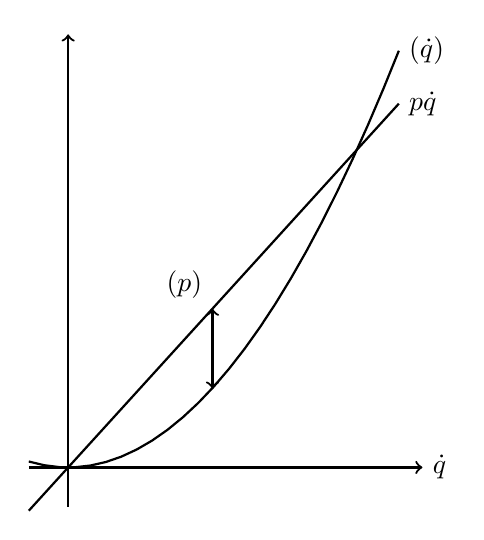
\begin{tikzpicture}
    \draw[->, thick] (-0.5, 0) -- (4.5, 0) node[anchor=west] {$\dot{q}$};
    \draw[->, thick] (0, -0.5) -- (0, 5.5);
    
    \draw[thick, domain=-0.5:4.2] plot ({\x}, {0.3*\x*\x}) node[anchor=west] {$\lag(\dot{q})$};
    \draw[thick, domain=-0.5:4.2] plot ({\x}, {1.1*\x}) node[anchor = west] {$p\dot{q}$};
    
    \draw[<->, thick] (1.8333, 1) -- (1.8333, 2.01663) node[anchor = south east] {$\ham(p)$};
    
\end{tikzpicture}
    \caption{Caption}
    \label{fig:my_label}
\end{figure}

\begin{econ}{The Legendre transform in economics}
    \towrite{TODO}
\end{econ}

\subsection{Hamilton's equations}
    \towrite{TODO}

\subsection{The canonical formalism}
One of the great advantages of Hamiltonian mechanics is that it admits a much wider range of coordinate transformations. Of course, any selection of the generalized coordinates that parameterizes the admissible motions of the system is equally valid, the generalized velocities are inherently tied to the choice of these coordinates. In Hamiltonian mechanics, the \(p\) and \(q\) coordinates can be chosen completely independent of each other, which is why a larger class of transformations is allowed\footnote{Due to the large variety of transformations, the coordinates for \(q\) and \(p\) may not longer just pertain to a `spatial' component and a `momentum' component, this distinction will then just be a matter of definition.} \cite{Landau1960}.

Canonical transformations are transformations such that Hamilton's equations remain valid in the new coordinate system. As shown by \citet{Landau1960}, each canonical transformation is characterized by a \emph{generating function}. Poisson brackets are invariant with respect to canonical transformations.

\subsection{Action-angle coordinates}
\towrite{TODO}

\subsection{Noether's theorem}
Conservation principles play a vital role in physics and mechanics. Notable examples are the conservation of energy, linear momentum, angular momentum and charge. A surprising result in physics is that all of the mentioned conservation laws are a consequence of the same theorem, attributed to Emmy Noether. This theorem essentially looks at the nature of the Lagrangian of the system, and sees whether it is `ignorant' with respect to certain group of transformations. As defined by \citet{Arnold1989}, the theorem is as follows:

\begin{thmblock}{Noether's theorem}
    If the Lagrangian system $(M, \lag)$ admits the one-parameter group of transformations $h^s: M \to M, s \in \real$, then the Lagrangian system of equations corresponding to $\lag$ has a first integral: $I: TM \to \real$. In local coordinates $q$ on $M$ the integral $I$ is written in teh form 
    $$ \left. I(\gpos, \gvel, t) = \pdv{\lag}{\gvel}\dv{h^s(\gpos)}{s}\right |_{s = 0} $$
\end{thmblock}
The word `admits' here means that the Lagrangian is invariant with respect to the transformation $h$; that is, the $\lag$ exhibits a \emph{symmetry} in that regard. A perspicuous consequence of this theorem is that when the Lagrangian has a cyclic coordinate (that is, it does not depend on some $q_i$), then the conjugate momentum of that coordinate is conserved, for the conjugate momentum of a coordinate $q_i$ is $\pdv{\lag}{\dot{q}_i}$.

\paragraph{Energy conservation} When the Lagrangian is time-invariant, one can define $h^s: (\gpos, t) \mapsto (\gpos, t + s)$ as translation in time. To find the conserved quantity, the Lagrangian has to be extended to consider the time $t$ as an explicit generalized coordinate, i.e. define
$$ \tilde{\lag}\qty(\gpos, t, \dv{\gpos}{\tau}, \dv{t}{\tau}) \triangleq \lag\qty(\gpos, \frac{\dv*{\gpos}{\tau}}{\dv*{t}{\tau}}, t)\dv{t}{\tau},$$
where $\tau$ now plays the role of the independent variable. This definition ensures that the action integral for $\tilde{\lag}$ and $\lag$ are identical, which is why Noether's theorem can be applied to $\tilde{\lag}$ instead. Of course, $\dv{h}{s}$ equal to 1 for the time coordinate; so there is one first integral
\begin{equation*}
    \begin{split}
        I = \pdv{\tilde{\lag}}{(t')} 
        &= \lag + \pdv{}{t'}\qty(\lag\qty(\gpos, \frac{
        \gpos'}{t'}, t))t'\\
        &= \lag + \pdv{\lag}{\gvel}\pdv{}{t'}\qty(\frac{
        \gpos'}{t'})t' = \lag - \pdv{\lag}{\gvel}\frac{\gpos'}{t'}\\
        &= \lag - \pdv{\lag}{\gvel}\gvel
    \end{split}
\end{equation*}
with $t' = \dv{t}{\tau}$ and $\gpos' = \dv{\gpos}{\tau}$. This is the negative of the Legendre transform of the Lagrangian, or the negative of the Hamiltonian; $I = -H$. Therefore, the total energy of the system is conserved. 

\paragraph{(Angular) momentum conservation} The invariance of the Lagrangian in one or more coordinate directions implies the conservation of the associated conjugate momentum. 

For example, a common assumption on Earth is that the gravitational force is constant and acts downwards. Therefore, only one coordinate appears in the potential energy expression, which is why the other coordinate directions (that is, the two `horizontal' directions, with proper choice of coordinate system) are cyclic. Hence, by virtue of Noether's theorem, the linear momentum in those directions is conserved, for it is unaffected by any potential force.

Conservation of angular momentum often appears in the presence of so-called \emph{central} force fields, which means that the potential energy is a function of the \emph{distance} from a certain point: notable examples are Coulomb forces or gravitational forces in celestial mechanics. Because only distance matters, the orientation of the displacement vector between the origin of the force field and the body is of no importance; it will not appear in the Lagrangian either. Consequently, Noether's theorem dictates that these central force fields preserve angular momentum.


\begin{econ}{Noether's theorem and conservation in economics}
    Noether's theorem can be applied to economic systems as well. The most simple application is the conservation of prices in the absence of scarcity. When the utility Lagrangian does not depend on a certain stock level $q_i$, that essentially means that there is no utility associated with the possession (or shortage) of it; in other words, economic agents are not driven by scarcity (or abundance) of that particular product. The `conjugate momentum' of an economic good is its price; so \emph{in the absence of scarcity, price is conserved}.\\
    
    A similar comment about cyclic coordinates can be made in the rotational analogy (which is to be discussed in \cref{chap:finance_rotation}). If the utility Lagrangian is independent on the return or interest $\zeta$, then borrowers or lenders will be indifferent about the realized returns of their investments, and never capitalize them (or in the case of borrowers, never repay their debts).\\
    
    Finally, the conservation of income in the economic system is related to the time-invariance of its Lagrangian. The Lagrangian does not depend on time if (i) there are no external influences or forcing terms and (ii) all parameters in the system remain constant over time. If that is the case, the Hamiltonian (or total income) in the economic system is conserved; or volume in the phase space (i.e. total amount of money) is conserved.\\
    
    Admittedly, all of these interpretations are arguably rather straightforward, since they mostly rely on either the presence cyclic coordinates or the direct correspondence of total energy and energy of the system. However, the discussion does prove that Noether's theorem has very tangible interpretations in economics. Its real power will, though, appear with more sophisticated symmetries that are present in complex economic systems. The idea is that the Lagrangian and Noether's theorem permit to extract `stylized facts' from these type of systems that would otherwise be concealed by their complexity. 
\end{econ}

